
% neue Folie
\newpage
\slidetitle{}
\section{Lindenmayer-Systeme \\}

\begin{itemize}
	\item Von Aristid Lindenmayer 1968 entwickelte Erweiterung von Ersetzungssystemen \\
	
	\item Weitere Ergänzungen durch Prusinkiewicz und Lindenmayer in 1990\\
	
	\item Funktionsweise basiert auf der Ersetzung von Zeichen in Zeichenketten \\
	
	\item Grafische Interpretation der Resultate ergibt Modelldaten
	
\end{itemize}

\newpage
\slidetitle{2. L-Systeme - D0L-Systeme}

\subsection{D0L-Systeme\\ }
\newtheorem{defD0LSystem}{Definition D0L-System:}[section]
\begin{defD0LSystem}
	Ein deterministisches, kontextfreies L-System (D0L-System) ist ein Tupel G = $(V, P, \omega)$, bestehend aus:
	
	\begin{description}
		\item[\boldmath$V$ ] Einem nichtleeren, endlichen Alphabet.\\
		
		\item[\boldmath$P$ ] Einer endlichen Menge von Produktionsregeln in der Form $P: a \rightarrow b$ mit $a \in V$ und $b \in V^*$. \\
		
		\item[\boldmath$\omega \in V^+$ ]  Dem Axiom, Startwort des L-Systems.		
	\end{description}
\end{defD0LSystem}

\newpage

\paragraph{Verwendete Begriffe:\\}

\begin{description}
	\item[\textbf{Deterministisch:}] Es existiert genau eine Produktionsregel für alle Symbole in $V$ \\
	
	\item[\textbf{Kontextfrei:}] Ersetzung findet unabhängig von umgebenden Symbolen statt \\
	
	\item[\textbf{Ableitung:}] Gleichzeitige Ersetzung aller Symbole eines Wortes anhand der Produktionsregeln
	
\end{description}

\newpage
\slidetitle{2. L-Systeme - D0L-Systeme}

\paragraph{Beispiel: Simulation des Wachstums der Blaualgen-Gattung \glqq Anabaena\grqq{} \\}

  
\begin{description}
	\item[\boldmath$V$]  besteht aus den Symbolen \boldmath$\{a_l, a_r, b_l, b_r\}$
	\begin{description}
		\item[\boldmath$a$ und \boldmath$b$:] Größe und Teilungsbereitschaft einer Zelle\\
		\item[\boldmath$l$ und \boldmath$r$:] Zellenpolarität
	\end{description}
	\item[\boldmath$P$] besteht aus:
	\begin{description}
		\item[\boldmath$p_1 :$] $\begin{array}{ccc} a_r & \rightarrow & a_lb_r \end{array}$
		\item[\boldmath$p_2 :$] $\begin{array}{ccc} a_l &\rightarrow& b_la_r \end{array}$
		\item[\boldmath$p_3 :$] $\begin{array}{ccc} b_r &\rightarrow& a_r \end{array}$
		\item[\boldmath$p_4 :$] $\begin{array}{ccc} b_l &\rightarrow& a_l  \end{array}$
	\end{description}
\end{description}

\newpage

\begin{center}
	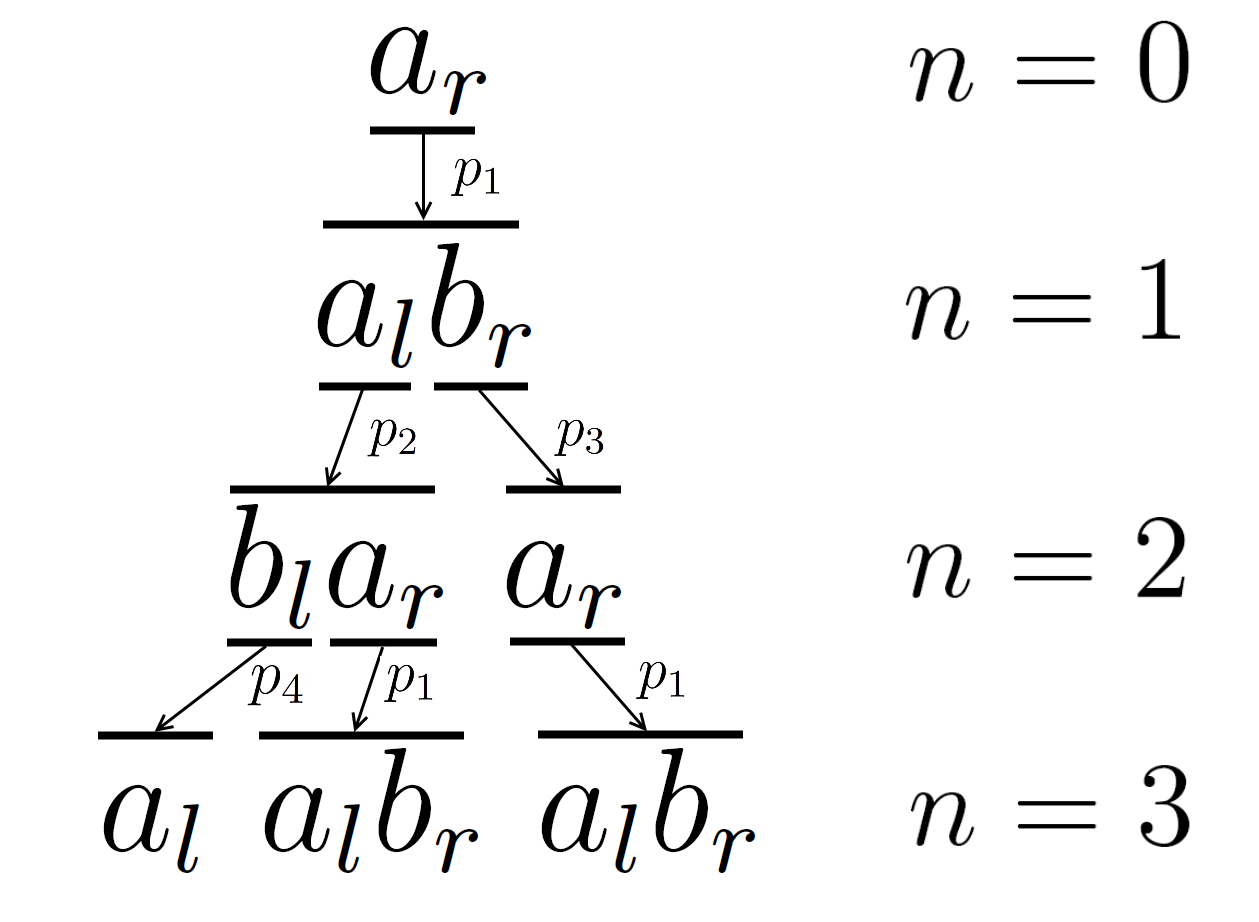
\includegraphics[height=1\textheight]{images/AnabaenaAbleitung.png}
\end{center}

\newpage
\slidetitle{2. L-Systeme - parametrische L-Systeme}
\subsection{Parametrische L-Systeme\\ }

\begin{itemize}
	\item Erweiterung der D0L-Systeme \\
	
	\item Verwendung von parametrischen Wörtern:
	\begin{description}
			\item[\boldmath$A(a_1, ..., a_n):$] Parametrisches Wort mit $A\in V$ und $a_1, ..., a_n \in \mathbb{R}$
	\end{description}
	
	\item 
	\begin{description}
		\item[\boldmath$\Sigma:$] Menge formaler Parameter
		\item[\boldmath$E(\Sigma):$] Arithmetischer Ausdruck
	\end{description}

	\item 
\end{itemize}

